%TODO: Use LaTeX_Header
\documentclass{article}
\iffalse
This file is protected by Copyright. Please refer to the COPYRIGHT file
distributed with this source distribution.

This file is part of OpenCPI <http://www.opencpi.org>

OpenCPI is free software: you can redistribute it and/or modify it under the
terms of the GNU Lesser General Public License as published by the Free Software
Foundation, either version 3 of the License, or (at your option) any later
version.

OpenCPI is distributed in the hope that it will be useful, but WITHOUT ANY
WARRANTY; without even the implied warranty of MERCHANTABILITY or FITNESS FOR A
PARTICULAR PURPOSE. See the GNU Lesser General Public License for more details.

You should have received a copy of the GNU Lesser General Public License along
with this program. If not, see <http://www.gnu.org/licenses/>.
\fi

\author{} % Force author to be blank
%----------------------------------------------------------------------------------------
% Paper size, orientation and margins
%----------------------------------------------------------------------------------------
\usepackage{geometry}
\geometry{
	letterpaper,			% paper type
	portrait,				% text direction
	left=.75in,				% left margin
	top=.75in,				% top margin
	right=.75in,			% right margin
	bottom=.75in			% bottom margin
 }
%----------------------------------------------------------------------------------------
% Header/Footer
%----------------------------------------------------------------------------------------
\usepackage{fancyhdr} \pagestyle{fancy} % required for fancy headers
\renewcommand{\headrulewidth}{0.5pt}
\renewcommand{\footrulewidth}{0.5pt}
\rhead{\small{OpenCPI}}
%----------------------------------------------------------------------------------------
% Appendix packages
%----------------------------------------------------------------------------------------
\usepackage[toc,page]{appendix}
%----------------------------------------------------------------------------------------
% Defined Commands & Renamed Commands
%----------------------------------------------------------------------------------------
\renewcommand{\contentsname}{Table of Contents}
\renewcommand{\listfigurename}{List of Figures}
\renewcommand{\listtablename}{List of Tables}
%----------------------------------------------------------------------------------------
% Various pacakges
%----------------------------------------------------------------------------------------
\usepackage{hyperref} % for linking urls and lists
\usepackage{graphicx} % for including pictures by file
\usepackage{listings} % for coding language styles
\usepackage{rotating} % for sideways table
\usepackage{pifont}   % for sideways table
\usepackage{pdflscape} % for landscape view
\usepackage{longtable}
%----------------------------------------------------------------------------------------
% Table packages
%----------------------------------------------------------------------------------------
\usepackage{tabularx} % c=center,l=left,r=right,X=fill
\usepackage{float}
\floatstyle{plaintop}
\usepackage[tableposition=top]{caption}
\newcolumntype{P}[1]{>{\centering\arraybackslash}p{#1}}
\newcolumntype{M}[1]{>{\centering\arraybackslash}m{#1}}
%----------------------------------------------------------------------------------------
% Block Diagram / FSM Drawings
%----------------------------------------------------------------------------------------
\usepackage{tikz}
\usetikzlibrary{shapes,arrows,fit,positioning}
\usetikzlibrary{automata} % used for the fsm
%----------------------------------------------------------------------------------------
% Colors Used
%----------------------------------------------------------------------------------------
\usepackage{colortbl}
\definecolor{blue}{rgb}{.7,.8,.9}
\definecolor{ceruleanblue}{rgb}{0.16, 0.32, 0.75}
\definecolor{drkgreen}{rgb}{0,0.6,0}
\definecolor{deepmagenta}{rgb}{0.8, 0.0, 0.8}
\definecolor{cyan}{rgb}{0.0,0.6,0.6}
\definecolor{maroon}{rgb}{0.5,0,0}

\usepackage{fancyvrb}
%\usepackage{glossaries}

%----------------------------------------------------------------------------------------
% Update the docTitle and docVersion per document
%----------------------------------------------------------------------------------------
\def\docTitle{Component Data Sheet}
\def\docVersion{1.5}
%----------------------------------------------------------------------------------------
\date{Version \docVersion} % Force date to be blank and override date with version
\title{\docTitle}
\lhead{\small{\docTitle}}

\def\snippetpath{snippets}
% Usage:
% \def\snippetpath{../../../../../doc/av/tex/snippets/}
% % Usage:
% \def\snippetpath{../../../../../doc/av/tex/snippets/}
% % Usage:
% \def\snippetpath{../../../../../doc/av/tex/snippets/}
% \input{\snippetpath/includes}
% From then on, you can use "input" With no paths to get to "snippets"
% You also get all "major" snippets not part of the global LaTeX_Header
% NOTE: If not using the global LaTeX_Header, you need to
% \usepackage{ifthen} to use the \githubio macro

\hyphenation{ANGRY-VIPER} % Tell it where to hyphenate
\hyphenation{Cent-OS} % Tell it where to hyphenate
\hyphenation{install-ation} % Tell it where to hyphenate

\newcommand{\todo}[1]{\textcolor{red}{TODO: #1}\PackageWarning{TODO:}{#1}} % To do notes
\newcommand{\code}[1]{\texttt{#1}} % For inline code snippet or command line
\newcommand{\sref}[1]{Section~\ref{#1}} % To quickly reference a section

% To quickly reference a versioned PDF on gitlab.io
\def\ocpiversion{develop}

% This gives a link to gitlab.io document. By default, it puts the filename.
% You can optionally change the link, e.g.
% \githubio{FPGA\_Vendor\_Tools\_Installation\_Guide.pdf} vs.
% \githubio[\textit{FPGA Vendor Tools Installation Guide}]{FPGA\_Vendor\_Tools\_Installation\_Guide.pdf}
% or if you want the raw ugly URL to come out, \githubioURL{FPGA_Vendor_Tools_Installation_Guide.pdf}
\newcommand{\githubio}[2][]{% The default is for FIRST param!
\href{http://opencpi.gitlab.io/releases/\ocpiversion/docs/#2}{\ifthenelse{\equal{#1}{}}{\texttt{#2}}{#1}}}
\newcommand{\gitlabcom}[2][]{% The default is for FIRST param!
\href{http://gitlab.com/opencpi/#2}{\ifthenelse{\equal{#1}{}}{\texttt{#2}}{#1}}}
\newcommand{\githubioURL}[1]{\url{http://opencpi.gitlab.io/releases/\ocpiversion/docs/#1}}
% Lastly, if you want a SINGLE leading path stripped, e.g. assets/X.pdf => X.pdf:
\newcommand{\githubioFlat}[1]{%
\StrBehind{#1}{/}[\den]%
\href{http://opencpi.gitlab.io/releases/\ocpiversion/docs/#1}{\texttt{\den}}%
}

% Fix import paths
\makeatletter
\def\input@path{{\snippetpath/}}
\makeatother

% From then on, you can use "input" With no paths to get to "snippets"
% You also get all "major" snippets not part of the global LaTeX_Header
% NOTE: If not using the global LaTeX_Header, you need to
% \usepackage{ifthen} to use the \githubio macro

\hyphenation{ANGRY-VIPER} % Tell it where to hyphenate
\hyphenation{Cent-OS} % Tell it where to hyphenate
\hyphenation{install-ation} % Tell it where to hyphenate

\newcommand{\todo}[1]{\textcolor{red}{TODO: #1}\PackageWarning{TODO:}{#1}} % To do notes
\newcommand{\code}[1]{\texttt{#1}} % For inline code snippet or command line
\newcommand{\sref}[1]{Section~\ref{#1}} % To quickly reference a section

% To quickly reference a versioned PDF on gitlab.io
\def\ocpiversion{develop}

% This gives a link to gitlab.io document. By default, it puts the filename.
% You can optionally change the link, e.g.
% \githubio{FPGA\_Vendor\_Tools\_Installation\_Guide.pdf} vs.
% \githubio[\textit{FPGA Vendor Tools Installation Guide}]{FPGA\_Vendor\_Tools\_Installation\_Guide.pdf}
% or if you want the raw ugly URL to come out, \githubioURL{FPGA_Vendor_Tools_Installation_Guide.pdf}
\newcommand{\githubio}[2][]{% The default is for FIRST param!
\href{http://opencpi.gitlab.io/releases/\ocpiversion/docs/#2}{\ifthenelse{\equal{#1}{}}{\texttt{#2}}{#1}}}
\newcommand{\gitlabcom}[2][]{% The default is for FIRST param!
\href{http://gitlab.com/opencpi/#2}{\ifthenelse{\equal{#1}{}}{\texttt{#2}}{#1}}}
\newcommand{\githubioURL}[1]{\url{http://opencpi.gitlab.io/releases/\ocpiversion/docs/#1}}
% Lastly, if you want a SINGLE leading path stripped, e.g. assets/X.pdf => X.pdf:
\newcommand{\githubioFlat}[1]{%
\StrBehind{#1}{/}[\den]%
\href{http://opencpi.gitlab.io/releases/\ocpiversion/docs/#1}{\texttt{\den}}%
}

% Fix import paths
\makeatletter
\def\input@path{{\snippetpath/}}
\makeatother

% From then on, you can use "input" With no paths to get to "snippets"
% You also get all "major" snippets not part of the global LaTeX_Header
% NOTE: If not using the global LaTeX_Header, you need to
% \usepackage{ifthen} to use the \githubio macro

\hyphenation{ANGRY-VIPER} % Tell it where to hyphenate
\hyphenation{Cent-OS} % Tell it where to hyphenate
\hyphenation{install-ation} % Tell it where to hyphenate

\newcommand{\todo}[1]{\textcolor{red}{TODO: #1}\PackageWarning{TODO:}{#1}} % To do notes
\newcommand{\code}[1]{\texttt{#1}} % For inline code snippet or command line
\newcommand{\sref}[1]{Section~\ref{#1}} % To quickly reference a section

% To quickly reference a versioned PDF on gitlab.io
\def\ocpiversion{develop}

% This gives a link to gitlab.io document. By default, it puts the filename.
% You can optionally change the link, e.g.
% \githubio{FPGA\_Vendor\_Tools\_Installation\_Guide.pdf} vs.
% \githubio[\textit{FPGA Vendor Tools Installation Guide}]{FPGA\_Vendor\_Tools\_Installation\_Guide.pdf}
% or if you want the raw ugly URL to come out, \githubioURL{FPGA_Vendor_Tools_Installation_Guide.pdf}
\newcommand{\githubio}[2][]{% The default is for FIRST param!
\href{http://opencpi.gitlab.io/releases/\ocpiversion/docs/#2}{\ifthenelse{\equal{#1}{}}{\texttt{#2}}{#1}}}
\newcommand{\gitlabcom}[2][]{% The default is for FIRST param!
\href{http://gitlab.com/opencpi/#2}{\ifthenelse{\equal{#1}{}}{\texttt{#2}}{#1}}}
\newcommand{\githubioURL}[1]{\url{http://opencpi.gitlab.io/releases/\ocpiversion/docs/#1}}
% Lastly, if you want a SINGLE leading path stripped, e.g. assets/X.pdf => X.pdf:
\newcommand{\githubioFlat}[1]{%
\StrBehind{#1}{/}[\den]%
\href{http://opencpi.gitlab.io/releases/\ocpiversion/docs/#1}{\texttt{\den}}%
}

% Fix import paths
\makeatletter
\def\input@path{{\snippetpath/}}
\makeatother


\def\comp{dig\_radio\_ctrlr}
\def\Comp{Digital Radio Controller}
\graphicspath{ {figures/} }

\begin{document}

\section*{Summary - \Comp}
\begin{longtable}{|p{\dimexpr0.5\textwidth-2\tabcolsep\relax}
                  |p{\dimexpr0.5\textwidth-2\tabcolsep\relax}|}
	\hline
	\rowcolor{blue}
	                  &                                        \\
	\hline
	Package Prefix    & ocpi.core \\
	\hline
	Name              & \comp                                  \\
	\hline
	OpenCPI Release Version & v\docVersion ~(release date 4/2019) \\
	\hline
\end{longtable}

\begin{center}
  \textit{\textbf{Revision History}}
  \begin{longtable}{|p{\dimexpr0.15\textwidth-2\tabcolsep\relax}
                    |p{\dimexpr0.65\textwidth-2\tabcolsep\relax}
                    |p{\dimexpr0.2\textwidth-2\tabcolsep\relax}|}
    \hline
    \rowcolor{blue}
    \textbf{Revision} & \textbf{Description of Change} & \textbf{Date} \\
    \hline
    v1.5 & Initial Release & 4/2019 \\
    \hline
  \end{longtable}
\end{center}

\section{Block Diagrams}

\begin{center}
  \begin{tikzpicture}[% List of styles applied to all, to override specify on a case-by-case
      every node/.style={
        align=center,     % use this so that the "\\" for line break works
        minimum size=2cm  % creates space above and below text in rectangle
      },
      every edge/.style={draw,thick}
    ]
    \node[rectangle,ultra thick,draw=black,fill=blue](R2){Parameter Properties:
\verb+MAX_STRING_LENGTH_p+, \\
\verb+NUM_DATA_STREAM_IDS_p+,
\verb+NUM_DATA_STREAM_IDS_RX_p+,
\verb+NUM_DATA_STREAM_IDS_TX_p+, \\
\verb+DATA_STREAM_IDS_RX_p+,
\verb+DATA_STREAM_IDS_TX_p+, \\
\verb+MAX_NUM_DATA_STREAMS_RX_p+,
\verb+MAX_NUM_DATA_STREAMS_TX_p+, \\
\verb+MIN_ACHIEVABLE_RX_TUNING_FREQ_MHZ_p+,
\verb+MAX_ACHIEVABLE_RX_TUNING_FREQ_MHZ_p+, \\
\verb+MIN_ACHIEVABLE_RX_BANDWIDTH_3DB_MHZ_p+,
\verb+MAX_ACHIEVABLE_RX_BANDWIDTH_3DB_MHZ_p+, \\
\verb+MIN_ACHIEVABLE_RX_SAMPLING_RATE_MSPS_p+,
\verb+MAX_ACHIEVABLE_RX_SAMPLING_RATE_MSPS_p+, \\
\verb+IS_SUPPORTED_RX_SAMPLES_COMPLEX_p+,
\verb+IS_SUPPORTED_RX_SAMPLES_REAL_p+, \\
\verb+IS_SUPPORTED_RX_GAIN_MODE_AUTO_p+,
\verb+IS_SUPPORTED_RX_GAIN_MODE_MANUAL_p+, \\
\verb+MIN_ACHIEVABLE_TX_TUNING_FREQ_MHZ_p+,
\verb+MAX_ACHIEVABLE_TX_TUNING_FREQ_MHZ_p+, \\
\verb+MIN_ACHIEVABLE_TX_BANDWIDTH_3DB_MHZ_p+,
\verb+MAX_ACHIEVABLE_TX_BANDWIDTH_3DB_MHZ_p+, \\
\verb+MIN_ACHIEVABLE_TX_SAMPLING_RATE_MSPS_p+,
\verb+MAX_ACHIEVABLE_TX_SAMPLING_RATE_MSPS_p+, \\
\verb+IS_SUPPORTED_TX_SAMPLES_COMPLEX_p+,
\verb+IS_SUPPORTED_TX_SAMPLES_REAL_p+ \\ \\
\Comp \\};
    \node[rectangle,draw=white,fill=white](R5)[above= of R2]{
      Non-parameter Properties: \verb+request_config_lock+, \\
      \verb+config_locks+, \\ \verb+unlock_config_lock+, \\
      \verb+unlock_all+, \\ \verb+data_stream_is_enabled+, \\
      \verb+direction_readback+, \\
      \verb+tuning_freq_MHz+, \\
      \verb+bandwidth_3dB_MHz+, \\ \verb+sampling_rate_Msps+, \\
      \verb+samples_are_complex+, \\ \verb+valid_values_tuning_freq_MHz+, \\
      \verb+valid_values_bandwidth_3dB_MHz+, \\
      \verb+valid_values_sampling_rate_Msps+, \\
      \verb+valid_values_samples_are_complex+ \\
      };
    \path[->]
    (R2)edge [] node [] {} (R5)
    (R5)edge [] node [] {} (R2)
    ;
  \end{tikzpicture}

\end{center}

\pagebreak

\tableofcontents

\pagebreak

\section{Functionality}

  \subsection{Digital Radio Controller Concept and Definition}

    \begin{center}
      \begin{figure}[h]
        \centering\captionsetup{type=figure}\includegraphics[scale=0.2]{dig_radio_ctrlr_minimal}
        \captionof{figure}{Digital Radio Controller - Major Concepts with Minimal Implementation.}
        \label{fig:blockdiagram}
      \end{figure}
    \end{center}

    \begin{center}
      \begin{figure}[h]
        \centering\captionsetup{type=figure}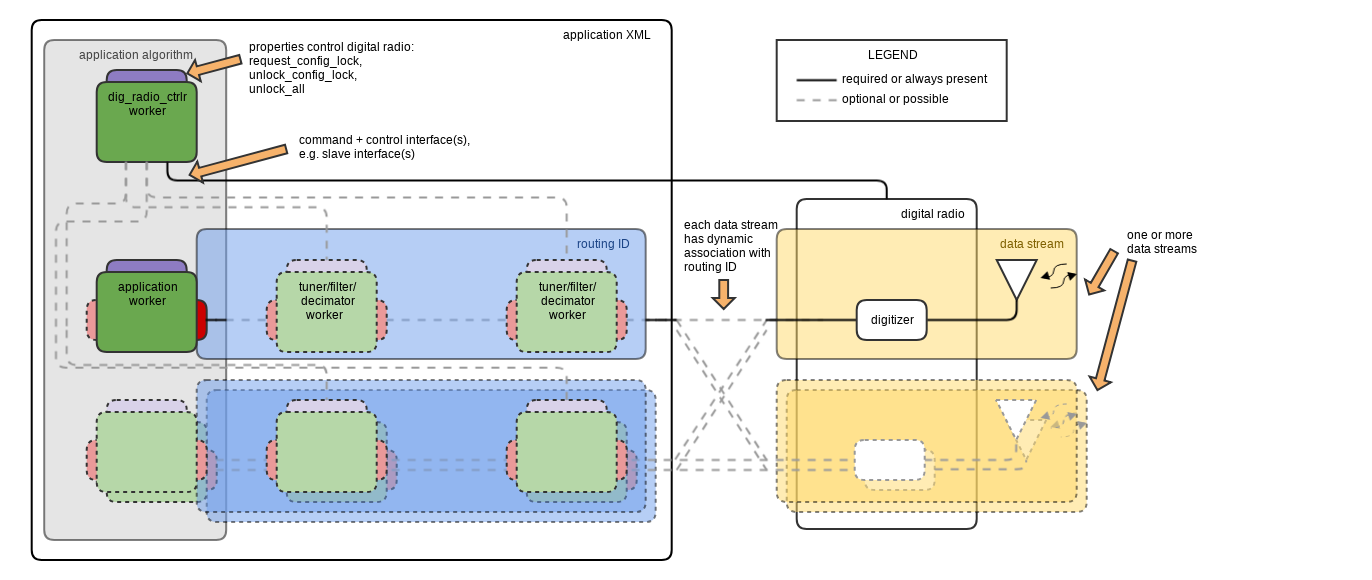
\includegraphics[scale=0.21]{dig_radio_ctrlr}
        \captionof{figure}{Digital Radio Controller - Major Concepts and Intended Usage.}
        \label{fig:blockdiagram}
      \end{figure}
    \end{center}
    \noindent Each worker implementing this component spec represents a
    \textit{digital radio controller}.
    A \textit{digital radio} exposes at least one worker port which streams digitized
    Radio Frequency (RF) samples within an OpenCPI application.
    Each port streams samples which were ultimately received (RX) from an ADC or will
    be transmitted (TX) to a DAC.
    Each port, including the characteristics of its RF
    source or destination, is represented as a \textit{data stream}.
    A \textit{digital radio controller} controls the configurations which
    characterize the RF source or destination of each
    \textit{data stream}'s samples, e.g. tuning
    frequency.
    Note that a \textit{digital radio controller} does not currently expose the
    ports which stream digitized samples.
    A \textit{digital radio controller} controls a single
    \textit{digital radio} and is capable of locking configurations to guarantee
    that their values cannot change. This locking mechanism is useful in
    guaranteeing that the act of configuring a \textit{data stream}
    does not
    corrupt the configuration of another \textit{data stream}. %, which is a
    %known shortcoming of the rx/tx component specs
    %implementations\cite{rx_tx_comp_datasheet}.
    In any given OpenCPI application, a
    \textit{digital radio controller} provides mechanisms for locking multiple
    \textit{data streams} of a single \textit{digital radio} at once as well as
    performing multiple successive locks and unlocks.

  \subsection{Data Stream Concept and Definition}
    A \textit{data stream} has the following characteristics.
    \begin{itemize}
      \item It corresponds to an RF data sink or source on the
            \textit{digital radio},
            usually an RF connector.
      \item It has an associated \textit{data stream ID}, which usually
            corresponds to the
            label of the RF connector it represents.
      \item It can be configured with at least one \textit{data stream type}
            which can be RX or TX. Workers implementing this spec are allowed to
            have a
            \textit{data stream} support both types, e.g. if the radio allows
            configuring a single RF connector for either RX or TX.
      \item It has, at a minimum, configurations for tuning frequency, 3dB bandwidth,
            and sampling rate, where:
      \begin{itemize}
        \item Tuning frequency is the RF frequency corresponding to 0 Hz in the
              baseband signal of the OpenCPI worker port which is exposed to
              the OpenCPI application's algorithm. This includes not only
              analog or digital tuning within the \textit{digital radio} but
              also any digital tuning that falls under control of the worker
              implementation of this component spec.
        \item The 3dB bandwidth is the maximum bandwidth for which the passband
              ripple can be reasonably guaranteed to be less than or equal to
              3dB for the combined filter response for all filtering that is
              applied between the RF spectrum and the OpenCPI worker port
              which is exposed to the OpenCPI application's algorithm. This
              includes not only analog or digital filtering within the
              \textit{digital radio} but also any digital filtering that falls
              under control of the worker which implements this component spec.
        \item The sampling rate is the rate at which the OpenCPI worker port
              which
              is exposed to the OpenCPI application's algorithm. This includes
              any digital upsampling or downsampling that falls under control of
              a worker which implements this component spec.
      \end{itemize}
    \end{itemize}

  \subsection{Routing ID Concept and Definition}
    While a \textit{data stream ID} corresponds to an RF data sink or source,
    a \textit{routing ID}
    associates a \textit{data stream ID} with an application-specific stream of
    OpenCPI workers. Because a \textit{digital radio} can have multiple
    \textit{data streams} of the same
    \textit{data stream type},
    it is possible that an application contains multiple workers whose
    connections are available to a given \textit{data stream}. The
    \textit{routing ID} disambiguates this association. At the moment, the worker
    implementations of this component define the intended labelling of
    \textit{routing IDs}. A \textit{routing ID} has the format RXn or TXn, where n is
    a zero-based index. For example, 'RX0' for
    a single-channel RX radio controller would always use 'RX0', and a
    dual-channel RX radio controller would allow 'RX0' or 'RX1'.

  \subsection{Configuration Lock Request Concept and Definition}
    Each \textit{digital radio controller}
    can be issued a \textit{config lock request}, which
    consists of a \textit{config lock ID} as well as
    requirements for one or more
    \textit{data streams}. The requirements for each \textit{data stream}
    include
    a \textit{routing ID} and a set of values and tolerances for that stream's
    configurations. The tolerances are used to determine
    if a lock was successful or not when applying rounding necessary for
    hardware configuration. Each \textit{config lock request} is expected to
    fail if the radio cannot support the requested values within the requested
    tolerances. When a \textit{config lock request} is successful, it is saved
    as
    \textit{config lock} whose values can be queried. Each \textit{config lock}
    can be
    unlocked, which requires a reference to its \textit{config lock ID}.

  %\subsection{Supporting C++ Classes}
  %  The assets projects' dig\_radio\_ctrlr\_fmcomms\_2\_3.rcc worker
  %  implementation\cite{dig_radio_ctrlr_fmcomms_2_3_comp_datasheet} of the
  %  \comp{}
  %  component spec includes C++ classes in support of the desired
  %  \comp{} functionality.
  %  Use of these classes is recommended for \comp{} worker
  %  implementations. The following classes are notable:
  %  \begin{itemize}
  %    \item \textit{ValidRanges} - This template class represents a collection of inclusive numeric ranges. 
  %    \item \textit{Configurator} - Software-only emulator of a hardware configuration environment which provides an API for locking/unlocking range-constrained configurations. Each configuration has a constraint which is a valid range represented by an object of the \textit{ValidRanges} type.
  %    \item \textit{DigRadioCtrlr} -
  %      Provides an API for controlling/locking analog and digital configs of
  %      a radio. When requesting config locks, a \textit{Configurator} object is
  %      queried for valid ranges before hardware actuation is performed.
  %  \end{itemize}
  %  If desired, doxygen documentation can be generated on all
  %  of the supporting classes in the dig\_radio\_ctlr\_fmcomms\_2\_3.rcc
  %  directory. Doxygen and
  %  either firefox or make and evince
  %  must be installed. To generate
  %  the documentation, run the following commands from the
  %  dig\_radio\_ctrlr\_fmcomms\_2\_3.rcc directory:
  %  \lstset{language=bash, backgroundcolor=\color{lightgray}, columns=flexible, breaklines=true, prebreak=\textbackslash, basicstyle=\ttfamily, showstringspaces=false,upquote=true, aboveskip=\baselineskip, belowskip=\baselineskip}
  %  \begin{lstlisting}
%cd ./supporting/
%doxygen
  %  \end{lstlisting}
%The generated HTML documentation can be viewed via:
  %  \begin{lstlisting}
%firefox ./html/index.html
  %  \end{lstlisting}
%The generated PDF documentation can be viewed via:
  %  \begin{lstlisting}
%make -C ./latex/
%evince ./latex/refman.pdf
  %  \end{lstlisting}

\subsection{Detailed Property Description}
  \label{sec:detailed_property_description}

  \subsubsection{Parameter Properties}
  \begin{itemize}
    \item \verb+MAX_STRING_LENGTH_p+
      \begin{itemize}
        \item Length of all string properties.
      \end{itemize}
    \item \verb+NUM_DATA_STREAM_IDS_p+
      \begin{itemize}
        \item Total number of \textit{data stream IDs}.
      \end{itemize}
    \item \verb+NUM_DATA_STREAM_IDS_RX_p+, \verb+NUM_DATA_STREAM_IDS_TX_p+
      \begin{itemize}
        \item Total number of \textit{data stream} IDs that can be configured
          for RX or
          TX
          streaming. Note this number of
          \textit{data streams} may not be available for use simultaneously.
          The purpose
          of
          these parameter properties is to provide the ability
          to enforce the array length of the
          \verb+DATA_STREAM_IDS_RX_p+
          parameter property.
      \end{itemize}
    \item \verb+DATA_STREAM_IDS_RX_p+, \verb+DATA_STREAM_IDS_TX_p+
      \begin{itemize}
        \item Defines all \textit{data streams} on the radio that can be
          configured for
          RX/TX streaming.
          Note that, of the streams specified in each of these parameter
          properties, only \\
          \verb+MAX_NUM_DATA_STREAMS_RX_p+/\verb+MAX_NUM_DATA_STREAMS_TX_p+
          number of
          the \textit{data streams} specified in this parameter property's are
          available
          for use
          simultaneously.
      \end{itemize}
    \item \verb+MAX_NUM_DATA_STREAMS_RX_p+, \verb+MAX_NUM_DATA_STREAMS_TX_p+
      \begin{itemize}
        \item Max number of simultaneously usable RX/TX \textit{data streams}
          available
          on radio.
          The purpose of these parameter properties is to provide the option for
          an OpenCPI
          application to use its selection feature\cite{ocpi_app_guide} to
          enforce
          application requirements of number of simultaneously usable
          RX/TX \textit{data streams} upon worker
          selection at runtime.
          %Either a worker's OWD or its build XML should
          %specify a value for each of these parameter properties.
    \end{itemize}
    \item \verb+MIN_ACHIEVABLE_RX_TUNING_FREQ_MHZ_p+,
      \verb+MAX_ACHIEVABLE_RX_TUNING_FREQ_MHZ_p+, \\
      \verb+MIN_ACHIEVABLE_RX_BANDWIDTH_3DB_MHZ_p+,
      \verb+MAX_ACHIEVABLE_RX_BANDWIDTH_3DB_MHZ_p+, \\
      \verb+MIN_ACHIEVABLE_RX_SAMPLING_RATE_MSPS_p+,
      \verb+MAX_ACHIEVABLE_RX_SAMPLING_RATE_MSPS_p+, \\
      \verb+MIN_ACHIEVABLE_TX_TUNING_FREQ_MHZ_p+,
      \verb+MAX_ACHIEVABLE_TX_TUNING_FREQ_MHZ_p+, \\
      \verb+MIN_ACHIEVABLE_TX_BANDWIDTH_3DB_MHZ_p+,
      \verb+MAX_ACHIEVABLE_TX_BANDWIDTH_3DB_MHZ_p+, \\
      \verb+MIN_ACHIEVABLE_TX_SAMPLING_RATE_MSPS_p+,
      \verb+MAX_ACHIEVABLE_TX_SAMPLING_RATE_MSPS_p+
      \begin{itemize}
        \item  Min/Max for all RX/TX \textit{data streams}.
          The purpose of these parameter properties is to provide the option for
          an OpenCPI
          application to use its selection feature\cite{ocpi_app_guide} to
          enforce
          application requirements of number of simultaneously usable
          RX/TX \textit{data streams} upon worker
          selection at runtime.
          %Either a worker's OWD or its build XML
          %should specify a value for each of these parameter properties.
      \end{itemize}
    \item \verb+IS_SUPPORTED_RX_SAMPLES_COMPLEX_p+,
      \verb+IS_SUPPORTED_RX_SAMPLES_REAL_p+, \\
      \verb+IS_SUPPORTED_RX_GAIN_MODE_AUTO_p+,
      \verb+IS_SUPPORTED_RX_GAIN_MODE_MANUAL_p+, \\
      \verb+IS_SUPPORTED_TX_SAMPLES_COMPLEX_p+,
      \verb+IS_SUPPORTED_TX_SAMPLES_REAL_p+
      \begin{itemize}
        \item True if supported by any RX/TX \textit{data streams}.
          The purpose of these parameter properties is to provide the option for
          an OpenCPI
          application to use its selection feature\cite{ocpi_app_guide} to
          enforce
          application requirements of number of simultaneously usable
          RX/TX \textit{data streams} upon worker
          selection at runtime.
          %Either a worker's OWD or its build XML
          %should specify a value for each of these parameter properties.
      \end{itemize}
  \end{itemize}

\pagebreak

\subsubsection{Non-Parameter Properties - request\_config\_lock}

  The \verb+request_config_lock+ property configures radio hardware for
  requested settings and prevents settings from changing thereafter. Struct
  members are
  as follows.

  \begin{itemize}
    \item config\_lock\_ID
      \begin{itemize}
        \item Each requested
              \textit{config lock}
              must have an associated ID which must be a
              non-empty string. If the request is successful, the locked values
              along with this ID are appended to the existing locks in the
              \verb+config_locks+ property, and this ID can
              be used in the future to unlock a specific lock.
      \end{itemize}
    \item data\_streams
      \begin{itemize}
        \item From 1 to (\verb+MAX_NUM_DATA_STREAMS_RX_p+ +
              \verb+MAX_NUM_DATA_STREAMS_TX_p+) data
              streams can be simultaneously requested to lock. This member is a
              sequence struct whose struct members are as follows.

          \begin{itemize}
            \item data\_stream\_type
              \begin{itemize}
                \item Set to RX or TX.
              \end{itemize}
            \item data\_stream\_ID
              \begin{itemize}
                \item Set to an empty string to request
                      \textit{data stream} by type only,
                      otherwise set to one of the values in \\
                      \verb+DATA_STREAM_IDS_RX_p+ or \verb+DATA_STREAM_IDS_TX_p+.
                      Requesting by type only means that any of the available
                      \textit{data streams}
                      which can be used for the given type could be used.
              \end{itemize}

            \item routing\_ID
              \begin{itemize}
                \item Usually set to "RXO', "TXO", "TX1",etc...
              \end{itemize}

            \item tuning\_freq\_MHz
            \item bandwidth\_3dB\_MHz
            \item sampling\_rate\_Msps
            \item samples\_are\_complex
            \item gain\_mode
              \begin{itemize}
                \item Set to "null", "auto", "manual", or possibly something
                      worker-specific.
                      A value of "null" means that a gain setting is not
                      included (ignored)
                      in the \textit{config lock request}
                      for the given \textit{data stream}, which means that
                      any gain setting which is present in the
                      \textit{data stream} will not be guaranteed.
                      Workers implementing this spec must always accept values of
                      "null", "auto", and "manual", but must fail if requests
                      for "auto" or "manual" are not supported by the
                      \textit{data stream}.
                      In additional, hardware-specific values are allowed to be
                      accepted by the worker.
              \end{itemize}

            \item gain\_dB
              \begin{itemize}
                \item If gain\_mode is "auto" or "null", this value will be ignored, i.e. a
                lock attempt for gain\_dB will not occur.
              \end{itemize}

            \item tolerance\_tuning\_freq\_MHz
              \begin{itemize}
                \item Tolerance which will determine lock success.
              \end{itemize}
            \item tolerance\_bandwidth\_3dB\_MHz
              \begin{itemize}
                \item Tolerance which will determine lock success.
              \end{itemize}
            \item tolerance\_sampling\_rate\_Msps
              \begin{itemize}
                \item Tolerance which will determine lock success.
              \end{itemize}

            \item tolerance\_gain\_dB
              \begin{itemize}
                \item Tolerance which will determine lock success.
                If gain\_mode is 'auto' or 'null', this value will be ignored, i.e. a
                lock attempt for gain\_dB will not occur.
              \end{itemize}
          \end{itemize}
      \end{itemize}
  \end{itemize}


  \subsubsection{Non-Parameter Properties - config\_locks}
  The \verb+config_locks+ property contains
  enumerations of currently locked configs for one or more
  \textit{data streams}.
  Struct
  members are as follows.
  \begin{itemize}
    \item \verb+config_lock_ID+
      \begin{itemize}
        \item ID of successfully requested \textit{config lock}.
      \end{itemize}
    \item \verb+data_streams+
      \begin{itemize}
        \item This member is a sequence of structs where the struct members are as follows.
          \begin{itemize}
            \item \verb+direction_lock+
              \begin{itemize}
                \item Locked \textit{data stream} type.
                  Value is for the \textit{data stream} specified in
                  \verb+data_stream_ID+.
              \end{itemize}
            \item \verb+data_stream_ID+
            \item \verb+routing_ID+
              \begin{itemize}
                \item Locked routing ID.
                  Value is for the \textit{data stream} specified in
                  \verb+data_stream_ID+.
              \end{itemize}
            \item \verb+tuning_freq_MHz+
              \begin{itemize}
                \item Locked tuning frequency.
                  Value is for the \textit{data stream} specified in
                  \verb+data_stream_ID+.
              \end{itemize}
            \item \verb+bandwidth_3dB_MHz+
              \begin{itemize}
                \item Locked 3dB bandwidth.
                  Value is for the \textit{data stream} specified in
                  \verb+data_stream_ID+.
              \end{itemize}
            \item \verb+sampling_rate_Msps+
              \begin{itemize}
                \item Locked sampling rate.
                  Value is for the \textit{data stream} specified in
                  \verb+data_stream_ID+.
              \end{itemize}
            \item \verb+samples_are_complex+
              \begin{itemize}
                \item Locked value.
                  Value is for the \textit{data stream} specified in
                  \verb+data_stream_ID+.
              \end{itemize}
            \item \verb+gain_mode_lock+
              \begin{itemize}
                \item Locked gain mode.
                  Value is for the \textit{data stream} specified in
                  \verb+data_stream_ID+.
              \end{itemize}
            \item \verb+gain_dB+
              \begin{itemize}
                \item Locked gain. Value should be ignored for auto gain modes.
                  Note that \verb+gain_mode_lock+ may have implementation-specific
                  auto gain modes in addition to the generic 'auto' mode.
                  Value is for the \textit{data stream} specified in
                  \verb+data_stream_ID+.
              \end{itemize}
          \end{itemize}

      \end{itemize}

  \end{itemize}

  \subsubsection{Non-Parameter Properties - unlock\_config\_lock}
  The \verb+unlock_config_lock+ property unlocks a \textit{config lock} by its
  ID. Struct
  members are as follows.
  \begin{itemize}
    \item \verb+config_lock_ID+
  \end{itemize}

  \subsubsection{Non-Parameter Properties - unlock\_all}
  The \verb+unlock_all+ property unlocks all existing \textit{config locks}.
  Write a
  value of true to this property to
  perform an unlock.

  \subsubsection{Non-Parameter Properties - Current Value Reading}
  The
  \verb+data_stream_is_enabled+,
  \verb+direction_readback+,
  \verb+tuning_freq_MHz+,
  \verb+bandwidth_3dB_MHz+, \\
  \verb+sampling_rate_Msps+, and 
  \verb+samples_are_complex+
  sequence properties are used to read the current config value
  (locked or not) for each enabled \textit{data stream}. Each
  sequence element contains the current config value for an enabled
  \textit{data stream}.
  Workers implementing this spec are expected to adjust this property's
  length such that it includes only enabled
  \textit{data streams}.
  If no
  \textit{data streams}
  are enabled, the sequence length is expected to be zero.

  \subsubsection{Non-Parameter Properties - Valid Values Reading}
  The
  \verb+valid_values_tuning_freq_MHz+,
  \verb+valid_values_bandwidth_3dB_MHz+,
  \verb+valid_values_sampling_rate_Msps+, and
  \verb+valid_values_samples_are_complex+
  array properties indicate the current valid ranges of
  values for all \textit{data streams}/\textit{data stream type}
  combinations.
  Each array element contains the
  ranges for a single \textit{data stream} for a single
  \textit{data stream type}.
  It is expected that \textit{data streams} that can be configured for either
  RX or TX will have a separate entry for each possible
  \textit{data stream type}.
  Once a config is locked, it
  is intended that its valid ranges will only consist of a single value.

\begin{landscape}

\section{Component Spec Property Table(s)}
  For a detailed property description, see \ref{sec:detailed_property_description}. \\ \\

	\noindent Table \hypertarget{tab1}{1}: Component Spec Properties.
	\begin{scriptsize}
		\begin{longtable}{|p{5.3cm}|c|p{3.5cm}|p{3.5cm}|c|c|p{4.4cm}|}
			\hline
			\rowcolor{blue}
			Name                                & Type   & Sequence & Array      & Accessibility       & Default & Description                                                                                \\
			\rowcolor{blue}
			                                    &        & Length   & Dimensions &                     &             &                                                                                            \\
			\hline
			\verb+MAX_STRING_LENGTH_p+ & UShort & -        & -          & Parameter           & 128     & Length of all string properties. \\
			\hline
			\verb+NUM_DATA_STREAM_IDS_p+           & UShort & -        & -          & Parameter           & 1       & Total number of \textit{data stream IDs}. \\
			\hline
			\verb+NUM_DATA_STREAM_IDS_RX_p+        & UShort & -        & -          & Parameter           & 1       & Total number of \textit{data stream IDs} that can be configured for RX streaming. \\
			\hline
			\verb+NUM_DATA_STREAM_IDS_TX_p+        & UShort & -        & -          & Parameter           & 1       & Total number of \textit{data stream IDs} that can be configured for TX streaming. \\
			\hline
			\verb+DATA_STREAM_IDS_RX_p+        & String & -        & \verb+NUM_DATA_STREAM_IDS_RX_p+ & Parameter           & -       & Defines all \textit{data streams} on the radio that can be configured for RX streaming. \\
			\hline
			\verb+DATA_STREAM_IDS_TX_p+        & String & -        & \verb+NUM_DATA_STREAM_IDS_TX_p+ & Parameter           & -       & Defines all \textit{data streams} on the radio that can be configured for TX streaming. \\
			\hline
			\verb+MAX_NUM_DATA_STREAMS_RX_p+        & UShort & -        & -          & Parameter           & 1       & Max number of simultaneously usable RX \textit{data streams} available on radio. \\
			\hline
			\verb+MAX_NUM_DATA_STREAMS_TX_p+        & UShort & -        & -          & Parameter           & 1       & Max number of simultaneously usable TX \textit{data streams} available on radio.  \\
			\hline
			\verb+MIN_ACHIEVABLE_RX_TUNING_FREQ_MHZ_p+        & Double & -        & - & Parameter          & -       & Min for all RX \textit{data streams}. \\
			\hline
			\verb+MAX_ACHIEVABLE_RX_TUNING_FREQ_MHZ_p+        & Double & -        & - & Parameter           & -       & Max for all RX \textit{data streams}. \\
			\hline
			\verb+MIN_ACHIEVABLE_RX_BANDWIDTH_3DB_MHZ_p+      & Double & -        & - & Parameter           & -       & Min for all RX \textit{data streams}. \\
			\hline
			\verb+MAX_ACHIEVABLE_RX_BANDWIDTH_3DB_MHZ_p+      & Double & -        & - & Parameter           & -       & Max for all RX \textit{data streams}. \\
			\hline
			\verb+MIN_ACHIEVABLE_RX_SAMPLING_RATE_MSPS_p+      & Double & -        & - & Parameter           & -       & Min for all RX \textit{data streams}. \\
			\hline
			\verb+MAX_ACHIEVABLE_RX_SAMPLING_RATE_MSPS_p+      & Double & -        & - & Parameter           & -       & Max for all RX \textit{data streams}. \\
			\hline
			\verb+IS_SUPPORTED_RX_SAMPLES_COMPLEX_p+           & Bool   & -        & - & Parameter           & -       & True if supported by any RX \textit{data streams}. \\
			\hline
			\verb+IS_SUPPORTED_RX_SAMPLES_REAL_p+              & Bool   & -        & - & Parameter           & -       & True if supported by any RX \textit{data streams}. \\
			\hline
			\verb+IS_SUPPORTED_RX_GAIN_MODE_AUTO_p+            & Bool   & -        & - & Parameter           & -       & True if supported by any RX \textit{data streams}. \\
			\hline
			\verb+IS_SUPPORTED_RX_GAIN_MODE_MANUAL_p+          & Bool   & -        & - & Parameter           & -       & True if supported by any RX \textit{data streams}. \\
			\hline
			\verb+MIN_ACHIEVABLE_TX_TUNING_FREQ_MHZ_p+        & Double & -        & - & Parameter           & -       & Min for all TX \textit{data streams}. \\
			\hline
			\verb+MAX_ACHIEVABLE_TX_TUNING_FREQ_MHZ_p+        & Double & -        & - & Parameter           & -       & Max for all TX \textit{data streams}. \\
			\hline
			\verb+MIN_ACHIEVABLE_TX_BANDWIDTH_3DB_MHZ_p+      & Double & -        & - & Parameter           & -       & Min for all TX \textit{data streams}. \\
			\hline
			\verb+MAX_ACHIEVABLE_TX_BANDWIDTH_3DB_MHZ_p+      & Double & -        & - & Parameter           & -       & Max for all TX \textit{data streams}. \\
			\hline
			\verb+MIN_ACHIEVABLE_TX_SAMPLING_RATE_MSPS_p+      & Double & -        & - & Parameter           & -       & Min for all TX \textit{data streams}. \\
			\hline
			\verb+MAX_ACHIEVABLE_TX_SAMPLING_RATE_MSPS_p+      & Double & -        & - & Parameter           & -       & Max for all TX \textit{data streams}. \\
			\hline
			\verb+IS_SUPPORTED_TX_SAMPLES_COMPLEX_p+           & Bool   & -        & - & Parameter           & -       & True if supported by any TX \textit{data streams}. \\
			\hline
			\verb+IS_SUPPORTED_TX_SAMPLES_REAL_p+              & Bool   & -        & - & Parameter           & -       & True if supported by any TX \textit{data streams}. \\
			\hline
			\verb+request_config_lock+          & Struct (see \hyperlink{tab2}{Table 2}) & - & -       & Writable    & -       & Configures radio hardware for requested settings and prevents settings from changing thereafter. \\
			\hline
			\verb+config_locks+                 & Struct (see \hyperlink{tab4}{Table 4}) & - & -       & Volatile & -       & Enumeration of currently locked configs. \\
			\hline
			\verb+unlock_config_lock+           & Struct (see \hyperlink{tab6}{Table 6}) & - & -       & Writable    & -       & Unlocks a \textit{config lock} by its ID. \\
			\hline
			\verb+unlock_all+                   & Bool & - & -       & Writable    & -       & Unlocks all existing \textit{config locks}. \\
			\hline
			\verb+data_stream_is_enabled+       & Struct (see \hyperlink{tab7}{Table 7}) & \verb+NUM_DATA_STREAM_IDS_p+ & - & Volatile    & -       & Used to read enabled status for all \textit{data streams}. \\
			\hline
			\verb+direction_readback+              & Struct (see \hyperlink{tab8}{Table 8}) & \verb+MAX_NUM_DATA_STREAMS_RX_p+ + \verb+MAX_NUM_DATA_STREAMS_TX_p+ & - &Volatile    & -       & Used to read current config value (locked or not) for each enabled \textit{data stream}. \\
			\hline
			\verb+tuning_freq_MHz+       & Struct (see \hyperlink{tab9}{Table 9}) & \verb+MAX_NUM_DATA_STREAMS_RX_p+ + \verb+MAX_NUM_DATA_STREAMS_TX_p+ & - &Volatile    & -       & Used to read current config value (locked or not) for each enabled \textit{data stream}. \\
			\hline
			\verb+bandwidth_3dB_MHz+     & Struct (see \hyperlink{tab10}{Table 10}) & \verb+MAX_NUM_DATA_STREAMS_RX_p+ + \verb+MAX_NUM_DATA_STREAMS_TX_p+ & - &Volatile    & -       & Used to read current config value (locked or not) for each enabled \textit{data stream}. \\
			\hline
			\verb+sampling_rate_Msps+    & Struct (see \hyperlink{tab11}{Table 11}) & \verb+MAX_NUM_DATA_STREAMS_RX_p+ + \verb+MAX_NUM_DATA_STREAMS_TX_p+ & - &Volatile    & -       & Used to read current config value (locked or not) for each enabled \textit{data stream}. \\
			\hline
			\verb+samples_are_complex+    & Struct (see \hyperlink{tab12}{Table 12}) & \verb+MAX_NUM_DATA_STREAMS_RX_p+ + \verb+MAX_NUM_DATA_STREAMS_TX_p+ & - &Volatile    & -       & Used to read current config value (locked or not) for each enabled \textit{data stream}. \\
			\hline
			\verb+valid_values_tuning_freq_MHz+    & Struct (see \hyperlink{tab13}{Table 13}) & - & \verb+NUM_DATA_STREAM_IDS_RX_p+ + \verb+NUM_DATA_STREAM_IDS_TX_p+ & Volatile    & -       & Indicates the current valid ranges of values for all \textit{data stream}/\textit{data stream type} combinations. \\
			\hline
			\verb+valid_values_bandwidth_3dB_MHz+    & Struct  (see \hyperlink{tab14}{Table 14})& - & \verb+NUM_DATA_STREAM_IDS_RX_p+ + \verb+NUM_DATA_STREAM_IDS_TX_p+ & Volatile    & -       & Indicates the current valid ranges of values for all \textit{data stream}/\textit{data stream type} combinations. \\
			\hline
			\verb+valid_values_sampling_rate_Msps+    & Struct  (see \hyperlink{tab15}{Table 15})& - & \verb+NUM_DATA_STREAM_IDS_RX_p+ + \verb+NUM_DATA_STREAM_IDS_TX_p+ & Volatile    & -       & Indicates the current valid ranges of values for all \textit{data stream}/\textit{data stream type} combinations. \\
			\hline
			\verb+valid_values_samples_are_complex+    & Struct  (see \hyperlink{tab16}{Table 16})& - & \verb+NUM_DATA_STREAM_IDS_RX_p+ + \verb+NUM_DATA_STREAM_IDS_TX_p+ & Volatile    & -       & Indicates the current valid ranges of values for all \textit{data stream}/\textit{data stream type} combinations. \\
			\hline

		\end{longtable}
	\end{scriptsize}

\pagebreak
	\noindent Table \hypertarget{tab2}{2}: Structure declaration for \comp{} \verb+request_config_lock+ property.
	\begin{scriptsize}
		\noindent\begin{longtable}{|p{1.8cm}|p{3.6cm}|c|p{4cm}|c|p{2cm}|p{1.7cm}|p{0.8cm}|p{3.10cm}|}
			\hline
			\rowcolor{blue}
			Type         & Name                                & Type & Sequence & Array      & Accessibility/ & Valid Range  & Default & Description                                                                                                                                                                                                                       \\
			\rowcolor{blue}
			             &                                     &      & Length   & Dimensions & Advanced       &              &         &                                                                                                                                                                                                                             \\
			\hline
			Member       & \verb+config_lock_ID+               & String& -       & -          & -              & Standard     & -       & ID used for future reference. \\
			\hline
			Member       & \verb+data_streams+                 & Struct (see \hyperlink{tab3}{Table 3}) & \verb+MAX_NUM_DATA_STREAMS_RX_p+ + \verb+MAX_NUM_DATA_STREAMS_TX_p+ & - & - & Standard & - & \\
			\hline
		\end{longtable}
	\end{scriptsize}

	\noindent Table \hypertarget{tab3}{3}: Structure declaration for \comp{} \verb+request_config_lock+ property's \verb+data_streams+ member. \\
	\begin{scriptsize}
		\noindent\begin{longtable}{|p{1.8cm}|p{3.6cm}|c|c|c|p{2cm}|p{1.7cm}|p{1.0cm}|p{7.37cm}|}
			\hline
			\rowcolor{blue}
			Type         & Name                                & Type & Sequence & Array      & Accessibility/ & Valid Range  & Default & Description                                                                                                                                                                                                                 \\
			\rowcolor{blue}
			             &                                     &      & Length   & Dimensions & Advanced       &              &         &                                                                                                                                                                                                                             \\
			\hline
			Member       & \verb+direction+                    & Enum  & -       & -          & -              & RX,TX        & -       & - \\
			\hline
			Member       & \verb+data_stream_ID+               & String& -       & -          & -              & Standard     & -       & Set to empty or to one of the values in \verb+DATA_STREAM_IDS_RX_p+ or \verb+DATA_STREAM_IDS_TX_p+. \\
			\hline
			Member       & \verb+routing_ID+                   & String& -       & -          & -              & Standard     & -       & Usually "RXO", "TX0", "TX1", etc... \\
			\hline
			Member       & \verb+tuning_freq_MHz+              & Double & -       & -          & -              & Standard     & -       & - \\
			\hline
			Member       & \verb+bandwidth_3dB_MHz+              & Double & -       & -          & -              & Standard     & -       & - \\
			\hline
			Member       & \verb+sampling_rate_Msps+             & Double & -       & -          & -              & Standard     & -       & - \\
			\hline
			Member       & \verb+samples_are_complex+            & Bool   & -       & -          & -              & Standard     & -       & - \\
			\hline
			Member       & \verb+gain_mode+                      & String & -       & -          & -              & Standard     & -       & Set to "null", "auto", "manual", or possibly something worker-specific. \\
			\hline
			Member       & \verb+gain_dB+                        & Double & -       & -          & -              & Standard     & -       & - \\
			\hline
			Member       & \verb+tolerance_tuning_freq_MHz+              & Double & -       & -          & -              & Standard     & -       & Tolerance which will determine lock success. \\
			\hline
			Member       & \verb+tolerance_bandwidth_3dB_MHz+              & Double & -       & -          & -              & Standard     & -       & Tolerance which will determine lock success. \\
			\hline
			Member       & \verb+tolerance_sampling_rate_Msps+             & Double & -       & -          & -              & Standard     & -       & Tolerance which will determine lock success. \\
			\hline
			Member       & \verb+tolerance_gain_dB+                        & Double & -       & -          & -              & Standard     & -       & Tolerance which will determine lock success. \\
			\hline
		\end{longtable}
	\end{scriptsize}

	\noindent Table \hypertarget{tab4}{4}: Structure declaration for \comp{} \verb+config_locks+ property.
	\begin{scriptsize}
		\noindent\begin{longtable}{|p{1.8cm}|p{3.6cm}|c|p{4cm}|c|p{2cm}|p{1.7cm}|p{0.8cm}|p{3.10cm}|}
			\hline
			\rowcolor{blue}
			Type         & Name                                & Type & Sequence & Array      & Accessibility/ & Valid Range  & Default & Description                                                                                                                                                                                                                       \\
			\rowcolor{blue}
			             &                                     &      & Length   & Dimensions & Advanced       &              &         &                                                                                                                                                                                                                             \\
			\hline
			Member       & \verb+config_lock_ID+               & String& -       & -          & -              & Standard     & -       & ID of successfully requested \textit{config lock}. \\
			\hline
			Member       & \verb+data_streams+                 & Struct (see \hyperlink{tab5}{Table 5}) & \verb+MAX_NUM_DATA_STREAMS_RX_p+ + \verb+MAX_NUM_DATA_STREAMS_TX_p+ & - & - & Standard & - & \\
			\hline
		\end{longtable}
	\end{scriptsize}

	\noindent Table \hypertarget{tab5}{5}: Structure declaration for \comp{} \verb+config_locks+ property's \verb+data_streams+ member. \\
	\begin{scriptsize}
		\noindent\begin{longtable}{|p{1.8cm}|p{3.6cm}|c|c|c|p{2cm}|p{1.7cm}|p{1.0cm}|p{7.38cm}|}
			\hline
			\rowcolor{blue}
			Type         & Name                                & Type & Sequence & Array      & Accessibility/ & Valid Range  & Default & Description                                                                                                                                                                                                                 \\
			\rowcolor{blue}
			             &                                     &      & Length   & Dimensions & Advanced       &              &         &                                                                                                                                                                                                                             \\
			\hline
			Member       & \verb+direction_lock+               & Enum  & -       & -          & -              & RX,TX        & -       & Locked type for \textit{data stream} specified in \verb+data_stream_ID+. \\
			\hline
			Member       & \verb+data_stream_ID+               & String& -       & -          & -              & Standard     & -       & - \\
			\hline
			Member       & \verb+routing_ID+                   & String& -       & -          & -              & Standard     & -       & Locked routing ID for \textit{data stream} specified in \verb+data_stream_ID+. \\
			\hline
			Member       & \verb+tuning_freq_MHz+              & Double & -       & -          & -              & Standard     & -       & Locked tuning frequency for \textit{data stream} specified in \verb+data_stream_ID+. \\
			\hline
			Member       & \verb+bandwidth_3dB_MHz+              & Double & -       & -          & -              & Standard     & -       & Locked 3dB bandwidth for \textit{data stream} specified in \verb+data_stream_ID+.- \\
			\hline
			Member       & \verb+sampling_rate_Msps+             & Double & -       & -          & -              & Standard     & -       & Locked sampling rate for \textit{data stream} specified in \verb+data_stream_ID+. \\
			\hline
			Member       & \verb+samples_are_complex+            & Bool   & -       & -          & -              & Standard     & -       & Locked value for \textit{data stream} specified in \verb+data_stream_ID+. \\
			\hline
			Member       & \verb+gain_mode_lock+                 & String & -       & -          & -              & Standard     & -       & Locked gain mode for \textit{data stream} specified in \verb+data_stream_ID+.- \\
			\hline
			Member       & \verb+gain_dB+                        & Double & -       & -          & -              & Standard     & -       & Ignore this value if \verb+gain_mode_lock+ is an AGC-related value, e.g. auto. \\
			\hline
		\end{longtable}
	\end{scriptsize}

	\noindent Table \hypertarget{tab6}{6}: Structure declaration for \comp{} \verb+unlock_config_lock+ property.
	\begin{scriptsize}
		\noindent\begin{longtable}{|p{1.8cm}|p{3.6cm}|c|p{4cm}|c|p{2cm}|p{1.7cm}|p{0.8cm}|p{4.81cm}|}
			\hline
			\rowcolor{blue}
			Type         & Name                                & Type & Sequence & Array      & Accessibility/ & Valid Range  & Default & Description                                                                                                                                                                                                                       \\
			\rowcolor{blue}
			             &                                     &      & Length   & Dimensions & Advanced       &              &         &                                                                                                                                                                                                                             \\
			\hline
			Member       & \verb+config_lock_ID+               & String& -       & -          & -              & Standard     & -       & - \\
			\hline
		\end{longtable}
	\end{scriptsize}

	\noindent Table \hypertarget{tab7}{7}: Structure declaration for \comp{} \verb+data_stream_is_enabled+ property.
	\begin{scriptsize}
		\noindent\begin{longtable}{|p{1.8cm}|p{3.6cm}|c|p{4cm}|c|p{2cm}|p{1.7cm}|p{0.8cm}|p{4.81cm}|}
			\hline
			\rowcolor{blue}
			Type         & Name                                & Type & Sequence & Array      & Accessibility/ & Valid Range  & Default & Description                                                                                                                                                                                                                       \\
			\rowcolor{blue}
			             &                                     &      & Length   & Dimensions & Advanced       &              &         &                                                                                                                                                                                                                             \\
			\hline
			Member       & \verb+data_stream_ID+               & String& -       & -          & -              & Standard     & -       & - \\
			\hline
			Member       & \verb+data_stream_is_enabled+       & Bool& -       & -          & -              & Standard & -       & - \\
			\hline
		\end{longtable}
	\end{scriptsize}

	\noindent Table \hypertarget{tab8}{8}: Structure declaration for \comp{} \verb+direction_readback+ property.
	\begin{scriptsize}
		\noindent\begin{longtable}{|p{1.8cm}|p{3.6cm}|c|p{4cm}|c|p{2cm}|p{1.7cm}|p{0.8cm}|p{4.81cm}|}
			\hline
			\rowcolor{blue}
			Type         & Name                                & Type & Sequence & Array      & Accessibility/ & Valid Range  & Default & Description                                                                                                                                                                                                                       \\
			\rowcolor{blue}
			             &                                     &      & Length   & Dimensions & Advanced       &              &         &                                                                                                                                                                                                                             \\
			\hline
			Member       & \verb+data_stream_ID+               & String& -       & -          & -              & Standard     & -       & - \\
			\hline
			Member       & \verb+direction_val+                & Bool& -       & -          & -              & Standard & -       & - \\
			\hline
		\end{longtable}
	\end{scriptsize}



	\noindent Table \hypertarget{tab9}{9}: Structure declaration for \comp{} \verb+tuning_freq_MHz+ property.
	\begin{scriptsize}
		\noindent\begin{longtable}{|p{1.8cm}|p{3.6cm}|c|p{4cm}|c|p{2cm}|p{1.7cm}|p{0.8cm}|p{4.69cm}|}
			\hline
			\rowcolor{blue}
			Type         & Name                                & Type & Sequence & Array      & Accessibility/ & Valid Range  & Default & Description                                                                                                                                                                                                                       \\
			\rowcolor{blue}
			             &                                     &      & Length   & Dimensions & Advanced       &              &         &                                                                                                                                                                                                                             \\
			\hline
			Member       & \verb+data_stream_ID+               & String& -       & -          & -              & Standard     & -       & - \\
			\hline
			Member       & \verb+tuning_freq_MHz+              & Double & -       & -          & -              & Standard & -       & - \\
			\hline
		\end{longtable}
	\end{scriptsize}

	\noindent Table \hypertarget{tab10}{10}: Structure declaration for \comp{} \verb+bandwidth_3dB_MHz+ property.
	\begin{scriptsize}
		\noindent\begin{longtable}{|p{1.8cm}|p{3.6cm}|c|p{4cm}|c|p{2cm}|p{1.7cm}|p{0.8cm}|p{4.69cm}|}
			\hline
			\rowcolor{blue}
			Type         & Name                                & Type & Sequence & Array      & Accessibility/ & Valid Range  & Default & Description                                                                                                                                                                                                                       \\
			\rowcolor{blue}
			             &                                     &      & Length   & Dimensions & Advanced       &              &         &                                                                                                                                                                                                                             \\
			\hline
			Member       & \verb+data_stream_ID+               & String& -       & -          & -              & Standard     & -       & - \\
			\hline
			Member       & \verb+bandwidth_3dB_MHz+            & Double & -       & -          & -              & Standard & -       & - \\
			\hline
		\end{longtable}
	\end{scriptsize}

	\noindent Table \hypertarget{tab11}{11}: Structure declaration for \comp{} \verb+sampling_rate_Msps+ property.
	\begin{scriptsize}
		\noindent\begin{longtable}{|p{1.8cm}|p{3.6cm}|c|p{4cm}|c|p{2cm}|p{1.7cm}|p{0.8cm}|p{4.69cm}|}
			\hline
			\rowcolor{blue}
			Type         & Name                                & Type & Sequence & Array      & Accessibility/ & Valid Range  & Default & Description                                                                                                                                                                                                                       \\
			\rowcolor{blue}
			             &                                     &      & Length   & Dimensions & Advanced       &              &         &                                                                                                                                                                                                                             \\
			\hline
			Member       & \verb+data_stream_ID+               & String& -       & -          & -              & Standard     & -       & - \\
			\hline
			Member       & \verb+sampling_rate_Msps+            & Double & -       & -          & -              & Standard & -       & - \\
			\hline
		\end{longtable}
	\end{scriptsize}

	\noindent Table \hypertarget{tab12}{12}: Structure declaration for \comp{} \verb+samples_are_complex+ property.
	\begin{scriptsize}
		\noindent\begin{longtable}{|p{1.8cm}|p{3.6cm}|c|p{4cm}|c|p{2cm}|p{1.7cm}|p{0.8cm}|p{4.81cm}|}
			\hline
			\rowcolor{blue}
			Type         & Name                                & Type & Sequence & Array      & Accessibility/ & Valid Range  & Default & Description                                                                                                                                                                                                                       \\
			\rowcolor{blue}
			             &                                     &      & Length   & Dimensions & Advanced       &              &         &                                                                                                                                                                                                                             \\
			\hline
			Member       & \verb+data_stream_ID+               & String& -       & -          & -              & Standard     & -       & - \\
			\hline
			Member       & \verb+samples_are_complex+           & Bool   & -       & -          & -              & Standard & -       & - \\
			\hline
		\end{longtable}
	\end{scriptsize}

	\noindent Table \hypertarget{tab13}{13}: Structure declaration for \comp{} \verb+valid_values_tuning_freq_MHz+ property.
	\begin{scriptsize}
		\noindent\begin{longtable}{|p{1.8cm}|p{3.6cm}|c|p{2cm}|c|p{2cm}|p{1.7cm}|p{0.8cm}|p{4.97cm}|}
			\hline
			\rowcolor{blue}
			Type         & Name                                & Type & Sequence & Array      & Accessibility/ & Valid Range  & Default & Description                                                                                                                                                                                                                       \\
			\rowcolor{blue}
			             &                                     &      & Length   & Dimensions & Advanced       &              &         &                                                                                                                                                                                                                             \\
			\hline
			Member       & \verb+data_stream_ID+               & String& -       & -          & -              & Standard     & -       & - \\
			\hline
			Member       & \verb+direction_tuning+             & Enum  & -       & -          & -              & RX,TX        & -       & - \\
			\hline
			Member       & \verb+valid_values+                 & Struct (see \hyperlink{tab17}{Table 17}) & 32      & -          & -              & Standard & -       & - \\
			\hline
		\end{longtable}
	\end{scriptsize}

	\noindent Table \hypertarget{tab14}{14}: Structure declaration for \comp{} \verb+valid_values_bandwidth_3dB_MHz+ property.
	\begin{scriptsize}
		\noindent\begin{longtable}{|p{1.8cm}|p{3.6cm}|c|p{2cm}|c|p{2cm}|p{1.7cm}|p{0.8cm}|p{4.97cm}|}
			\hline
			\rowcolor{blue}
			Type         & Name                                & Type & Sequence & Array      & Accessibility/ & Valid Range  & Default & Description                                                                                                                                                                                                                       \\
			\rowcolor{blue}
			             &                                     &      & Length   & Dimensions & Advanced       &              &         &                                                                                                                                                                                                                             \\
			\hline
			Member       & \verb+data_stream_ID+               & String& -       & -          & -              & Standard     & -       & - \\
			\hline
			Member       & \verb+direction_bandwidth+          & Enum  & -       & -          & -              & RX,TX        & -       & - \\
			\hline
			Member       & \verb+valid_values+                 & Struct (see \hyperlink{tab17}{Table 17}) & 32      & -          & -              & Standard & -       & - \\
			\hline
		\end{longtable}
	\end{scriptsize}

	\noindent Table \hypertarget{tab15}{15}: Structure declaration for \comp{} \verb+valid_values_sampling_rate_Msps+ property.
	\begin{scriptsize}
		\noindent\begin{longtable}{|p{1.8cm}|p{3.6cm}|c|p{2cm}|c|p{2cm}|p{1.7cm}|p{0.8cm}|p{4.97cm}|}
			\hline
			\rowcolor{blue}
			Type         & Name                                & Type & Sequence & Array      & Accessibility/ & Valid Range  & Default & Description                                                                                                                                                                                                                       \\
			\rowcolor{blue}
			             &                                     &      & Length   & Dimensions & Advanced       &              &         &                                                                                                                                                                                                                             \\
			\hline
			Member       & \verb+data_stream_ID+               & String& -       & -          & -              & Standard     & -       & - \\
			\hline
			Member       & \verb+direction_sampling+           & Enum  & -       & -          & -              & RX,TX        & -       & - \\
			\hline
			Member       & \verb+valid_values+                 & Struct (see \hyperlink{tab17}{Table 17}) & 32      & -          & -              & Standard & -       & - \\
			\hline
		\end{longtable}
	\end{scriptsize}

	\noindent Table \hypertarget{tab16}{16}: Structure declaration for \comp{} \verb+valid_values_samples_are_complex+ property.
	\begin{scriptsize}
		\noindent\begin{longtable}{|p{1.8cm}|p{3.6cm}|c|p{2cm}|c|p{2cm}|p{1.7cm}|p{0.8cm}|p{6.81cm}|}
			\hline
			\rowcolor{blue}
			Type         & Name                                & Type & Sequence & Array      & Accessibility/ & Valid Range  & Default & Description                                                                                                                                                                                                                       \\
			\rowcolor{blue}
			             &                                     &      & Length   & Dimensions & Advanced       &              &         &                                                                                                                                                                                                                             \\
			\hline
			Member       & \verb+data_stream_ID+               & String& -       & -          & -              & Standard     & -       & - \\
			\hline
			Member       & \verb+direction_samples_are+        & Enum  & -       & -          & -              & RX,TX        & -       & - \\
			\hline
			Member       & \verb+valid_values+                 & Bool  & 2       & -          & -              & Standard & -       & - \\
			\hline
		\end{longtable}
	\end{scriptsize}

	\noindent Table \hypertarget{tab17}{17}: Structure declaration for \comp{} \verb+valid_values_tuning_freq_MHz+, \verb+valid_values_bandwidth_3dB+, and \\ \verb+valid_values_sampling_rate_Msps+ property's \verb+valid_values+ members.
	\begin{scriptsize}
		\noindent\begin{longtable}{|p{1.8cm}|p{3.6cm}|c|p{4cm}|c|p{2cm}|p{1.7cm}|p{0.8cm}|p{4.69cm}|}
			\hline
			\rowcolor{blue}
			Type         & Name                                & Type & Sequence & Array      & Accessibility/ & Valid Range  & Default & Description                                                                                                                                                                                                                       \\
			\rowcolor{blue}
			             &                                     &      & Length   & Dimensions & Advanced       &              &         &                                                                                                                                                                                                                             \\
			\hline
			Member       & \verb+min+                          & Double & -       & -          & -              & Standard     & -       & - \\
			\hline
			Member       & \verb+max+                          & Double & -       & -          & -              & Standard     & -       & - \\
			\hline
		\end{longtable}
	\end{scriptsize}

\end{landscape}

%\makeglossaries

%\newglossaryentry{latex}
%{
%    name=latex,
%    description={Is a mark up language specially suited 
%    for scientific documents}
%}
 
%\newglossaryentry{maths}
%{
%    name=mathematics,
%    description={Mathematics is what mathematicians do}
%}

%\printglossaries

\begin{thebibliography}{1}

  \bibitem{dig_radio_ctrlr_fmcomms_2_3_comp_datasheet}
  \githubio[FMCOMMS2/3 Digital Radio Controller Worker]{assets/Dig\_Radio\_Ctrlr\_FMCOMMS\_2\_3.pdf} \\
  \bibitem{ocpi_app_guide}
  \githubio[OpenCPI Application Development]{OpenCPI\_Application\_Development.pdf}
  %\bibitem{rx_tx_comp_datasheet} Generic RF Interface \\
  %\url{https://opencpi.github.io/Generic_RF_Interface.pdf}

\end{thebibliography}

\end{document}
